\documentclass[a4paper]{article}

\usepackage[pdftex,
  hidelinks,
  pdfauthor={Dexter Chua},
  pdfsubject={Cambridge Maths Notes: Part IB - Electromagnetism},
  pdftitle={Part IB - Electromagnetism},
pdfkeywords={Cambridge Mathematics Maths Math IB Lent Electromagnetism}]{hyperref}

% Imports
\ifx \nextra \undefined
  \usepackage[pdftex,
    hidelinks,
    pdfauthor={Dexter Chua},
    pdfsubject={Cambridge Maths Notes: Part \npart\ - \ncourse},
    pdftitle={Part \npart\ - \ncourse},
  pdfkeywords={Cambridge Mathematics Maths Math \npart\ \nterm\ \nyear\ \ncourse}]{hyperref}
  \title{Part \npart\ - \ncourse}
\else
  \usepackage[pdftex,
    hidelinks,
    pdfauthor={Dexter Chua},
    pdfsubject={Cambridge Maths Notes: Part \npart\ - \ncourse\ (\nextra)},
    pdftitle={Part \npart\ - \ncourse\ (\nextra)},
  pdfkeywords={Cambridge Mathematics Maths Math \npart\ \nterm\ \nyear\ \ncourse\ \nextra}]{hyperref}

  \title{Part \npart\ - \ncourse \\ {\Large \nextra}}
\fi

\author{Lectured by \nlecturer \\\small Notes taken by Dexter Chua}
\date{\nterm\ \nyear}

\usepackage{alltt}
\usepackage{amsfonts}
\usepackage{amsmath}
\usepackage{amssymb}
\usepackage{amsthm}
\usepackage{booktabs}
\usepackage{caption}
\usepackage{enumitem}
\usepackage{fancyhdr}
\usepackage{graphicx}
\usepackage{mathtools}
\usepackage{microtype}
\usepackage{multirow}
\usepackage{pdflscape}
\usepackage{pgfplots}
\usepackage{siunitx}
\usepackage{tabularx}
\usepackage{tikz}
\usepackage{tkz-euclide}
\usepackage[normalem]{ulem}
\usepackage[all]{xy}

\pgfplotsset{compat=1.12}

\pagestyle{fancyplain}
\lhead{\emph{\nouppercase{\leftmark}}}
\ifx \nextra \undefined
  \rhead{
    \ifnum\thepage=1
    \else
      \npart\ \ncourse
    \fi}
\else
  \rhead{
    \ifnum\thepage=1
    \else
      \npart\ \ncourse\ (\nextra)
    \fi}
\fi
\usetikzlibrary{arrows}
\usetikzlibrary{decorations.markings}
\usetikzlibrary{decorations.pathmorphing}
\usetikzlibrary{positioning}
\usetikzlibrary{fadings}
\usetikzlibrary{intersections}
\usetikzlibrary{cd}

\newcommand*{\Cdot}{\raisebox{-0.25ex}{\scalebox{1.5}{$\cdot$}}}
\newcommand {\pd}[2][ ]{
  \ifx #1 { }
    \frac{\partial}{\partial #2}
  \else
    \frac{\partial^{#1}}{\partial #2^{#1}}
  \fi
}

% Theorems
\theoremstyle{definition}
\newtheorem*{aim}{Aim}
\newtheorem*{axiom}{Axiom}
\newtheorem*{claim}{Claim}
\newtheorem*{cor}{Corollary}
\newtheorem*{defi}{Definition}
\newtheorem*{eg}{Example}
\newtheorem*{fact}{Fact}
\newtheorem*{law}{Law}
\newtheorem*{lemma}{Lemma}
\newtheorem*{notation}{Notation}
\newtheorem*{prop}{Proposition}
\newtheorem*{thm}{Theorem}

\renewcommand{\labelitemi}{--}
\renewcommand{\labelitemii}{$\circ$}
\renewcommand{\labelenumi}{(\roman{*})}

\let\stdsection\section
\renewcommand\section{\newpage\stdsection}

% Strike through
\def\st{\bgroup \ULdepth=-.55ex \ULset}

% Maths symbols
\newcommand{\bra}{\langle}
\newcommand{\ket}{\rangle}

\newcommand{\N}{\mathbb{N}}
\newcommand{\Z}{\mathbb{Z}}
\newcommand{\Q}{\mathbb{Q}}
\renewcommand{\H}{\mathbb{H}}
\newcommand{\R}{\mathbb{R}}
\newcommand{\C}{\mathbb{C}}
\newcommand{\Prob}{\mathbb{P}}
\renewcommand{\P}{\mathbb{P}}
\newcommand{\E}{\mathbb{E}}
\newcommand{\F}{\mathbb{F}}
\newcommand{\cU}{\mathcal{U}}
\newcommand{\RP}{\mathbb{RP}}
\newcommand{\CP}{\mathbb{CP}}

\newcommand{\ph}{\,\cdot\,}

\DeclareMathOperator{\sech}{sech}
\DeclareMathOperator{\cosech}{cosech}
\DeclareMathOperator{\cosec}{cosec}

\DeclareMathOperator{\covol}{covol}
\DeclareMathOperator{\vol}{vol}

\let\Im\relax
\let\Re\relax
\DeclareMathOperator{\Im}{Im}
\DeclareMathOperator{\Re}{Re}
\DeclareMathOperator{\im}{im}
\DeclareMathOperator{\image}{image}
\DeclareMathOperator{\Ann}{Ann}

\DeclareMathOperator*{\res}{res}
\DeclareMathOperator{\Res}{Res}
\DeclareMathOperator{\Ind}{Ind}

\DeclareMathOperator{\tr}{tr}
\DeclareMathOperator{\diag}{diag}
\DeclareMathOperator{\rank}{rank}
\DeclareMathOperator{\card}{card}
\DeclareMathOperator{\spn}{span}
\DeclareMathOperator{\adj}{adj}

\DeclareMathOperator{\erf}{erf}
\DeclareMathOperator{\erfc}{erfc}

\DeclareMathOperator{\ord}{ord}
\DeclareMathOperator{\Sym}{Sym}

\DeclareMathOperator{\sgn}{sgn}
\DeclareMathOperator{\orb}{orb}
\DeclareMathOperator{\stab}{stab}
\DeclareMathOperator{\ccl}{ccl}

\DeclareMathOperator{\lcm}{lcm}
\DeclareMathOperator{\hcf}{hcf}

\DeclareMathOperator{\Int}{Int}
\DeclareMathOperator{\id}{id}

\DeclareMathOperator{\betaD}{beta}
\DeclareMathOperator{\gammaD}{gamma}
\DeclareMathOperator{\Poisson}{Poisson}
\DeclareMathOperator{\binomial}{binomial}
\DeclareMathOperator{\multinomial}{multinomial}
\DeclareMathOperator{\Bernoulli}{Bernoulli}
\DeclareMathOperator{\like}{like}

\DeclareMathOperator{\var}{var}
\DeclareMathOperator{\cov}{cov}
\DeclareMathOperator{\bias}{bias}
\DeclareMathOperator{\mse}{mse}
\DeclareMathOperator{\corr}{corr}

\DeclareMathOperator{\otp}{otp}
\DeclareMathOperator{\dom}{dom}

\DeclareMathOperator{\Root}{Root}
\DeclareMathOperator{\supp}{supp}
\DeclareMathOperator{\rel}{rel}
\DeclareMathOperator{\Hom}{Hom}
\DeclareMathOperator{\Aut}{Aut}
\DeclareMathOperator{\Gal}{Gal}
\DeclareMathOperator{\Mat}{Mat}
\DeclareMathOperator{\End}{End}
\DeclareMathOperator{\Char}{char}
\DeclareMathOperator{\ev}{ev}
\DeclareMathOperator{\St}{St}
\DeclareMathOperator{\Lk}{Lk}
\DeclareMathOperator{\disc}{disc}
\DeclareMathOperator{\Isom}{Isom}
\DeclareMathOperator{\length}{length}
\DeclareMathOperator{\energy}{energy}
\DeclareMathOperator{\area}{area}
\DeclareMathOperator{\Syl}{Syl}
\DeclareMathOperator{\cl}{cl}
\DeclareMathOperator{\fix}{fix}

\newcommand{\GL}{\mathrm{GL}}
\newcommand{\SL}{\mathrm{SL}}
\newcommand{\PGL}{\mathrm{PGL}}
\newcommand{\PSL}{\mathrm{PSL}}
\newcommand{\PSU}{\mathrm{PSU}}
\newcommand{\Or}{\mathrm{O}}
\newcommand{\SO}{\mathrm{SO}}
\newcommand{\U}{\mathrm{U}}
\newcommand{\SU}{\mathrm{SU}}

\renewcommand{\d}{\mathrm{d}}
\newcommand{\D}{\mathrm{D}}

\tikzset{->/.style = {decoration={markings,
                                  mark=at position 1 with {\arrow[scale=2]{latex'}}},
                      postaction={decorate}}}
\tikzset{<-/.style = {decoration={markings,
                                  mark=at position 0 with {\arrowreversed[scale=2]{latex'}}},
                      postaction={decorate}}}
\tikzset{<->/.style = {decoration={markings,
                                   mark=at position 0 with {\arrowreversed[scale=2]{latex'}},
                                   mark=at position 1 with {\arrow[scale=2]{latex'}}},
                       postaction={decorate}}}
\tikzset{->-/.style = {decoration={markings,
                                   mark=at position #1 with {\arrow[scale=2]{latex'}}},
                       postaction={decorate}}}
\tikzset{-<-/.style = {decoration={markings,
                                   mark=at position #1 with {\arrowreversed[scale=2]{latex'}}},
                       postaction={decorate}}}

\tikzset{circ/.style = {fill, circle, inner sep = 0, minimum size = 3}}
\tikzset{mstate/.style={circle, draw, blue, text=black, minimum width=0.7cm}}

\definecolor{mblue}{rgb}{0.2, 0.3, 0.8}
\definecolor{morange}{rgb}{1, 0.5, 0}
\definecolor{mgreen}{rgb}{0.1, 0.4, 0.2}
\definecolor{mred}{rgb}{0.5, 0, 0}

\def\drawcirculararc(#1,#2)(#3,#4)(#5,#6){%
    \pgfmathsetmacro\cA{(#1*#1+#2*#2-#3*#3-#4*#4)/2}%
    \pgfmathsetmacro\cB{(#1*#1+#2*#2-#5*#5-#6*#6)/2}%
    \pgfmathsetmacro\cy{(\cB*(#1-#3)-\cA*(#1-#5))/%
                        ((#2-#6)*(#1-#3)-(#2-#4)*(#1-#5))}%
    \pgfmathsetmacro\cx{(\cA-\cy*(#2-#4))/(#1-#3)}%
    \pgfmathsetmacro\cr{sqrt((#1-\cx)*(#1-\cx)+(#2-\cy)*(#2-\cy))}%
    \pgfmathsetmacro\cA{atan2(#2-\cy,#1-\cx)}%
    \pgfmathsetmacro\cB{atan2(#6-\cy,#5-\cx)}%
    \pgfmathparse{\cB<\cA}%
    \ifnum\pgfmathresult=1
        \pgfmathsetmacro\cB{\cB+360}%
    \fi
    \draw (#1,#2) arc (\cA:\cB:\cr);%
}
\newcommand\getCoord[3]{\newdimen{#1}\newdimen{#2}\pgfextractx{#1}{\pgfpointanchor{#3}{center}}\pgfextracty{#2}{\pgfpointanchor{#3}{center}}}

\def\Xint#1{\mathchoice
   {\XXint\displaystyle\textstyle{#1}}%
   {\XXint\textstyle\scriptstyle{#1}}%
   {\XXint\scriptstyle\scriptscriptstyle{#1}}%
   {\XXint\scriptscriptstyle\scriptscriptstyle{#1}}%
   \!\int}
\def\XXint#1#2#3{{\setbox0=\hbox{$#1{#2#3}{\int}$}
     \vcenter{\hbox{$#2#3$}}\kern-.5\wd0}}
\def\ddashint{\Xint=}
\def\dashint{\Xint-}


\title{Part IB - Electromagnetism}
\author{Lectured by David Tong}
\date{Lent 2015}

\begin{document}
\maketitle
{\small
\noindent\textbf{Electromagnetism and Relativity}\\
Review of Special Relativity; tensors and index notation. Lorentz force law. Electromagnetic tensor. Lorentz transformations of electric and magnetic fields. Currents and the conservation of charge. Maxwell equations in relativistic and non-relativistic forms.\hspace*{\fill} [5]

\vspace{10pt}
\noindent\textbf{Electrostatics}\\
Gauss's law. Application to spherically symmetric and cylindrically symmetric charge distributions.  Point, line and surface charges. Electrostatic potentials; general charge distributions, dipoles. Electrostatic energy. Conductors.\hspace*{\fill} [3]

\vspace{10pt}
\noindent\textbf{Magnetostatics}\\
Magnetic fields due to steady currents. Ampre's law. Simple examples. Vector potentials and the Biot-Savart law for general current distributions. Magnetic dipoles. Lorentz force on current distributions and force between current-carrying wires. Ohm's law.\hspace*{\fill} [3]

\vspace{10pt}
\noindent\textbf{Electrodynamics}\\
Faraday's law of induction for fixed and moving circuits. Electromagnetic energy and Poynting vector.  4-vector potential, gauge transformations. Plane electromagnetic waves in vacuum, polarization.\hspace*{\fill} [5]}

\tableofcontents
\section{Introduction}
Electromagnetism is important.
\subsection{Charge and Current}
The strength of the electromagnetic force experienced by a particle is determined by its \emph{(electric) charge}. The SI unit of charge is the \emph{Columb}. In this course, we assume that the charge can be any real number. However, at the fundamental level, charge is quantised. All particles carry charge $q = ne$ with $n\in \Z$, \footnote{Actually quarks have $n = \pm1/3$ or $\pm2/3$, but when we study quarks, electromagnetism becomes insignificant compared to the strong force. So for all practical purposes we can have $n\in \Z$.} and the basic unit $e \approx 1.6 \times 10^{-19} $C. For example, the electron has $n = -1$, proton has $n = +1$, neutron = $n = 0$.

In this course, it will be more useful to talk about \emph{charge density} $\rho(\mathbf{x}, t)$.
\begin{defi}[Charge density]
  The \emph{charge density} is the charge per unit volume. The total charge in a region $V$ is
  \[
    Q = \int_V \rho(\mathbf{x}, t)\; \d^3 x
  \]
\end{defi}

The motion of charge is described by the \emph{current} density $\mathbf{J}(\mathbf{x}, t)$.
\begin{defi}[Current and current density]
For any surface $S$, the integral
\[
  I = \int_S \mathbf{J}\cdot d\mathbf{S}
\]
counts the charge per unit time passing through $S$. $I$ is the \emph{current}, and $\mathbf{J}$ is the \emph{charge density}, ``current per unit area''.
\end{defi}
Intuitively, if the charge distribution $\rho (\mathbf{x}, t)$ has velocity $\mathbf{v}(x, t)$, then (neglecting relativistic effects), we have
\[
  \mathbf{J} = \rho \mathbf{v}
\]

\begin{eg}
  A wire is a cylinder of cross-sectional area $A$. Suppose there are $n$ electrons per unit volume. Then
  \begin{align*}
    \rho &= nq = -ne\\
    \mathbf{J} &= nq\mathbf{v}\\
    I &= nqvA
  \end{align*}
\end{eg}

It is well know that charge is conserved. However, we can have a stronger statement- charge is conserved locally: it is not possible that a charge in a box disappears and instantaneously appears on the moon. If it disappears in the box, it must have moved to somewhere nearby.

This is captured by the \emph{continuity equation}.
\begin{law}[Continuity equation]
  \[
    \frac{\partial\rho}{\partial t} + \nabla\cdot \mathbf{J} = 0
  \]
\end{law}
The charge $Q$ in some region $V$ is
\[
  Q = \int_V \rho \;\d^3 x
\]
So
\[
  \frac{\d Q}{\d t} = \int_V \frac{\partial\rho}{\partial t}\; d^3 x = -\int_V \nabla\cdot \mathbf{J}\; \d^3 x = -\int_S \mathbf{J}\cdot \d S
\]
where the last equality is by the divergence theorem. i.e. the rate of change in charge is the rate of charge flowing out of the point.

We can take $V = \R^3$, the whole of space. If there are no currents at infinity, then
\[
  \frac{\d Q}{\d t} = 0
\]
So the continuity equation implies the conservation of charge.

\subsection{Forces and Fields}
All forces are mediated by \emph{fields}. In physics a \emph{field} is a dynamical quantity which takes values at every point in space and time. The electromagnetic force is mediated by two fields:
\begin{itemize}
  \item electric field $\mathbf{E}(\mathbf{x}, t)$
  \item magnetic field $\mathbf{B}(\mathbf{x}, t)$
\end{itemize}
Each of these fields is itself a 3-vector. There are two aspects to the force:
\begin{itemize}
  \item Particles create fields
  \item Fields move particles
\end{itemize}
The second aspect is governed by the Lorentz force law:
\begin{law}[Lorentz force law]
\[
  \mathbf{F} = q(\mathbf{E} + \mathbf{v}\times \mathbf{B})
\]
\end{law}
The first aspect is governed by \emph{Maxwell's equations}.
\begin{law}[Maxwell's Equations]
  \begin{align*}
    \nabla \cdot \mathbf{E} &= \frac{\rho}{\varepsilon_0}\\
    \nabla \cdot \mathbf{B} &= 0\\
    \nabla \times \mathbf{E} +\frac{\partial \mathbf{E}}{\partial t} &= 0\\
    \nabla \times \mathbf{B} - \mu_0\varepsilon_0 \frac{\partial \mathbf{E}}{\partial t} = \mu_0 \mathbf{j}
  \end{align*}
  where
  \begin{itemize}
    \item $\varepsilon_0 = \SI{8.85e-12}{\per\metre\cubed\per\kilogram\s\squared\coulomb\squared}$ is the electric constant
    \item $\mu_0 = \SI{4\pi e-6}{\metre\kilogram\per\coulomb\squared}$ is the magnetic constant
  \end{itemize}
\end{law}
These equations are special in a mathematical way. In fact, using quantum mechanics and relativity, it can be shown that these are the only equations that can possibly describe electromagnetism.

\section{Electrostatics}
Take a stationary charge density $\rho = \rho(\mathbf{x})$ with $\mathbf{J} = 0$. We look for time-independent solutions with $\mathbf{B} = 0$. We are left with two equations
\begin{align*}
  \nabla \cdot \mathbf{E} &= \frac{\rho}{\varepsilon_0}\\
  \nabla\times \mathbf{E} &= 0
\end{align*}
and the other two equations just give $0 = 0$. Our goal is: Given $\rho$, find $\mathbf{E}$.
\subsection{Gauss' Law}
Consider a region $V\subseteq \R^3$ with boundary $S = \partial V$. We integrate the first equation over $V$:
\[
  \int \nabla\cdot \mathbf{E}\; \d^3 x = \int_S \mathbf{E}\cdot \d \mathbf{S} = \frac{1}{\varepsilon_0} \int_V \rho \;\d ^3 x.
\]
So
\begin{law}[Gauss' law]
  \[
    \int_S \mathbf{E}\cdot \d \mathbf{S} =\frac{Q}{\varepsilon_0},
  \]
  where $Q$ is the total charge inside $V$.
\end{law}
\begin{defi}[Flux through surface]
  The \emph{flux} of $\mathbf{E}$ through the surface $S$ is defined to be 
  \[
    \int_S \mathbf{E} \cdot\d \mathbf{S}.
  \]
\end{defi}

\note All surfaces containing charge $Q$ have the same flux. Only charge inside $S$ contributes to the flux. If there is a charge outside, then the field lines go in through one side of the surface and leave through the other. Then it gives no total flux.

From this, we can prove Columb's law:
\begin{eg}
  Gauss' law $\Rightarrow$ Columb's force law.

  We consider a spherically symmetric charge density $\rho (r)$. with $\rho (r) = 0$ for $r > R$, i.e. all the charge is contained in a ball of radius $R$.

  \begin{center}
    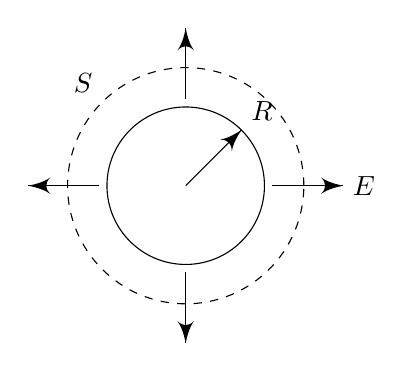
\begin{tikzpicture}
      \draw circle [radius=1];
      \draw [->] (0, 0) -- (.71, .71) node [anchor=south west] {$R$};
      \draw [->] (0, 1.1) -- (0, 2);
      \draw [->] (0, -1.1) -- (0, -2);
      \draw [->] (1.1, 0) -- (2, 0) node [right] {$E$};
      \draw [->] (-1.1, 0) -- (-2, 0);
      \draw [dashed] circle [radius=1.5];
      \node at (-1.06, 1.06) [anchor=south east] {$S$};
    \end{tikzpicture}
  \end{center}

  By symmetry, the force is the same in all directions and point outward radially. So
  \[
    \mathbf{E} = E(r) \hat{\mathbf{r}}.
  \]
  This immediately ensures that $\nabla \times \mathbf{E} = 0$.

  Put $S$ to be a sphere of radius $r > R$. Then
  \begin{align*}
    \int_S \mathbf{E}\cdot \d \mathbf{S} &= \int_S E(r) \hat{\mathbf{r}}\cdot \d \mathbf{S}\\
    &= E(r) \int_S \hat{\mathbf{r}}\cdot \d \mathbf{S}\\
    &= E(r)\cdot 4\pi r^2\\
    &= \frac{Q}{\varepsilon_0}
  \end{align*}
  We were able to pull the $E(r)$ out since it is constant over the sphere.

  Therefore
  \[
    \mathbf{E}(r) = \frac{Q}{4\pi\varepsilon_0 r^2}\hat{\mathbf{r}}.
  \]
  The Lorentz force law tells us that the force experienced by a second charge is
  \[
    \mathbf{F}(\mathbf{r}) = \frac{Qq}{4\pi\varepsilon_0 r^2}\hat{\mathbf{r}},
  \]
  which is Columb's law. Note that strictly speaking, this only holds when the charges are not moving. However, we can still use this because the corrections when they move are tiny.
\end{eg}

\begin{eg}
  Consider a uniform sphere with
  \[
    \rho (r) = \begin{cases}
      \rho & r < R\\
      0 & r > R
    \end{cases}.
  \]
  Outside, we know that 
  \[
    \mathbf{E} = \frac{Q}{4\pi\varepsilon_0 r^2}\hat{\mathbf{r}}
  \]

  Now suppose we are inside the sphere.
   \begin{center}
    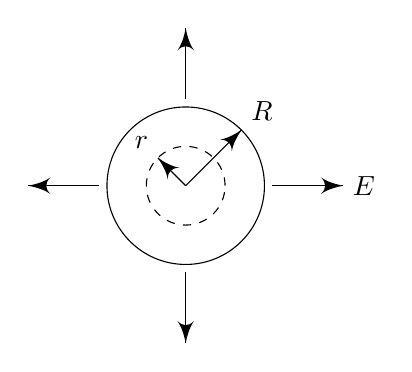
\begin{tikzpicture}
      \draw circle [radius=1];
      \draw [->] (0, 0) -- (.71, .71) node [anchor=south west] {$R$};
      \draw [->] (0, 1.1) -- (0, 2);
      \draw [->] (0, -1.1) -- (0, -2);
      \draw [->] (1.1, 0) -- (2, 0) node [right] {$E$};
      \draw [->] (-1.1, 0) -- (-2, 0);
      \draw [dashed] circle [radius=0.5];
      \draw [->] (0, 0) -- (-.353, .353) node [anchor=south east] {$r$};
    \end{tikzpicture}
  \end{center}

  Then
  \begin{align*}
    \int_S \mathbf{E}\cdot \d\mathbf{S} &= E(r) 4\pi r^2\\
    &= \frac{Q}{\varepsilon_0}\left(\frac{r^3}{R^3}\right)
  \end{align*}
  
  So 
  \[
    \mathbf{E}(r) = \frac{Qr}{4\pi\varepsilon_0 R^3}\hat{\mathbf{r}},
  \]
  and the field increases with radius. 
\end{eg}

\begin{eg}[Line charge]
  Consider an infinite line with uniform charge density \emph{per unit length} $\eta$.

  We use cylindrical polar coordinates:
  \begin{center}
    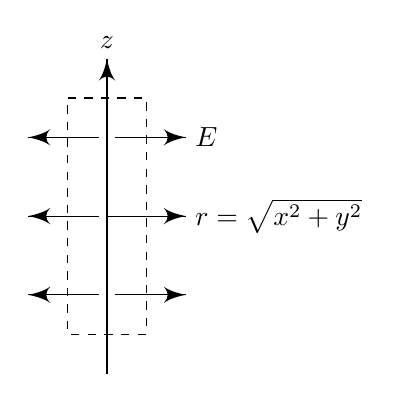
\begin{tikzpicture}
      \draw [->] (0, -2) -- (0, 2) node [above] {$z$};
      \draw [->] (0, 0) -- (1, 0) node [right] {$r = \sqrt{x^2 + y^2}$};

      \draw [->] (0.1, 1) -- (1, 1) node [right] {$E$};
      \draw [->] (-0.1, 1) -- (-1, 1);
      \draw [->] (-0.1, 0) -- (-1, 0);
      \draw [->] (0.1, -1) -- (1, -1);
      \draw [->] (-0.1, -1) -- (-1, -1);

      \draw [dashed] (-0.5, 1.5) -- (0.5, 1.5) -- (0.5, -1.5) -- (-0.5, -1.5) -- cycle;
    \end{tikzpicture}
  \end{center}

  By symmetry, the field is radial, i.e.
  \[
    \mathbf{E}(r) = E(r) \hat{\mathbf{r}}.
  \]
  Pick $S$ to be a cylinder of length $L$ and radius $r$. We know that the end caps do not contribute to the flux since the field lines are perpendicular to the normal. Then
  \[
    \int_S\mathbf{E}\cdot \mathbf{S} = E(r)2\pi rL = \frac{\eta L}{\varepsilon_0}.
  \]
  So
  \[
    \mathbf{E}(r) = \frac{\eta}{2\pi \varepsilon_0 r} \hat{\mathbf{r}}.
  \]
  Note that the field varies as $1/r$, not $1/r^2$. Intuitively, this is because we have one more dimension of ``stuff'' compared to the point charge. 
\end{eg}

\begin{eg}[Surface charge]
  Consider an infinite plane $z = 0$, with uniform charge per unit area $\sigma$.

  \begin{center}
    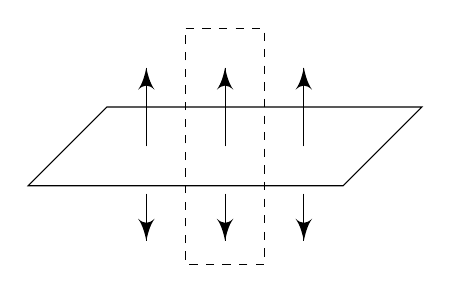
\begin{tikzpicture}
      \draw (-2.5, -.5) -- (1.5, -.5) -- (2.5, .5) -- (-1.5, .5) -- cycle;
      \draw [->] (0, 0) -- (0, 1);
      \draw [->] (-1, 0) -- (-1, 1);
      \draw [->] (1, 0) -- (1, 1);
      
      \draw [->] (0, -.6) -- (0, -1.2);
      \draw [->] (1, -.6) -- (1, -1.2);
      \draw [->] (-1, -.6) -- (-1, -1.2);

      \draw [dashed] (-0.5, 1.5) -- (0.5, 1.5) -- (0.5, -1.5) -- (-0.5, -1.5) -- cycle;
    \end{tikzpicture}
  \end{center}

  By symmetry, the field points vertically, and the field bottom is the opposite of that on top. we must have
  \[
    \mathbf{E} = E(z)\hat{\mathbf{z}}
  \]
  with
  \[
    E(z) = -E(-z).
  \]
  Consider a vertical cylinder of height $2z$ and cross-sectional area $A$. Now only the end caps contribute.
  \begin{align*}
    \int_S \mathbf{E} \cdot \d \mathbf{S} &= E(z) A - E(-z) A\\
    &=\frac{\sigma A}{\varepsilon _0}. 
  \end{align*}
  So
  \[
    E(z) = \frac{\sigma }{2\varepsilon_0}
  \]
  and is constant.

  Note that the electric field is discontinuous across the surface. We have
  \[
    E(z\to 0+) - E(z\to 0-) = \frac{\sigma}{\varepsilon_0}.
  \]
  Note that this is a general result that is true for any arbitrary surfaces and $\sigma$. We can prove this by considering a cylinder across the surface and then shrink it indefinitely. The we find that
  \[
    \hat{\mathbf{n}}\cdot \mathbf{E}_+ - \hat{\mathbf{n}}\cdot \mathbf{E}_- = \frac{\sigma}{\varepsilon_0}.
  \]
  However, the components of $\mathbf{E}$ tangential to the sruface are continuous. 
\end{eg}
\end{document}
